\section{Subadditive Valuations}
\label{sec:SubaddVal}

In this section we present our main technical result which establishes the existence of $1/2$-MMS allocation for the case of at most four agents (Theorem~\ref{thm:mainTheorem}). In Sections~\ref{sec:2Subadd}-~\ref{sec:4Subadd} we establish the existence of $1/2$-MMS approximate allocations for two, three and four subadditive agents (Corollaries~\ref{cor:2agents},~\ref{cor:3agents}~and~\ref{cor:4agents}), respectively, that follow as simple corollaries from more restricted settings (Lemmas~\ref{Lemma:2agents}, \ref{Lemma:threehalfs}, and \ref{Lemma:4agents}, respectively). We note that all these results improve the state-of-the-art for MMS guarantees for a wide set of valuation classes that lie below subadditive in the complement-free hierarchy. Subsequently, in Section \ref{sec:MoreAgents} we show how our proof techniques can be extended to obtain positive results for settings with many agents, when the agents have one of two types of admissible valuation functions. We emphasize that all the results presented herein are tight for subadditive valuations, i.e., there exist constructions where not all agents can receive more than $1/2$ of their MMS values \cite{GhodsiHSSY22}. In the proofs which follow we use ``symmetric'' cuts, i.e. no matter if $\mathcal{X}^*_i(C)=\mathcal{X}_i(C)$ or $\mathcal{X}^*_i(C)=\mathcal{X}_i(M \setminus C)$ for the maximum desired half of agent $i$ over cut $C$, the proof will continue the same way. 


\begin{theorem}
\label{thm:mainTheorem}
    An $1/2$-MMS allocation exists for at most four agents with subadditive valuations.
\end{theorem}

Before proceeding with the proofs for few agents, we give the following general observation that illustrates the implications of our results. 

\begin{observation}
\label{obs:simpleReduction}
    Given some fair division instance, an allocation that is $\boldsymbol{\alpha}$-MMS$(\mathbf{d})$ is also $\boldsymbol{\alpha}'$-MMS$(\mathbf{d}')$, where $\boldsymbol{\alpha}$ is pointwise larger or equal to $\boldsymbol{\alpha}'$, and $\mathbf{d}$ is pointwise smaller or equal to $\mathbf{d}'$.
\end{observation}
\begin{proof}
    Let $A=(A_1,\ldots, A_n)$ be a $\boldsymbol{\alpha}$-MMS$(\mathbf{d})$ allocation. By definition it holds that for each agent $i$, $v_i(A_i)\geq \alpha_i \mu_i^{d_i}$. 
    
    We first show that $A$ is also a $\boldsymbol{\alpha}$-MMS$(\mathbf{d}')$ allocation.  
    Note that if for some agent $i$ there exists a partition of $M$ into $d_i'$ bundles that she values each by at least $\mu_i^{d_i'}$, then there exists a partition into $d_i\le d_i'$ bundles that she values by at least the same amount, by merging bundles of the first partition, due to monotonicity of the valuation functions. This in turns implies that $\mu_i^{d_i}\geq \mu_i^{d_i'}$. Therefore, $v_i(A_i)\geq \alpha_i \mu_i^{d_i'}$, for all $i$, which implies that $A$ is a $\boldsymbol{\alpha}$-MMS$(\mathbf{d}')$ allocation. 
    
    To complete the proof, it simply holds that $v_i(A_i)\geq \alpha_i \mu_i^{d_i'}\ge \alpha_i' \mu_i^{d_i'}$, for all $i$, which means that $A$ is also a $\boldsymbol{\alpha}'$-MMS$(\mathbf{d}')$ allocation. 
\end{proof}


\subsection{Two Agents}
\label{sec:2Subadd}
In this section we show that there always exists a $1/2$-MMS allocation for the case of two agents. We first show a stronger statement (Lemma~\ref{Lemma:2agents}) and obtain the main result as a corollary (Corollary~\ref{cor:2agents}). We further provide a useful restatement (Corollary~\ref{Cor:cut-and-choose}) of Lemma~\ref{Lemma:2agents} to be extensively used in the proofs for three and four agents.

\begin{lemma}[Two agents]
\label{Lemma:2agents}
    A $(1/2,1)$-MMS$(1,2)$ allocation exists for two agents with subadditive valuation functions. 
\end{lemma}


\begin{proof}


    We denote by $S$ and $T$ the two agents and by $S_j, T_j$ their $j$-th MMS bundle respectively, i.e., $S_1$ for the first agent and $T_1, T_2$ for the second agent. 
    We proceed in a cut-and-choose fashion; we partition the set of items into two disjoint bundles $T_1, T_2$ which both are worth at least $1$ for $T$. Agent $S$ picks her favorite bundle which (due to subadditivity) is guaranteed to have at least $1/2$ value since $v_S(T_1) + v_S(T_2) \geq v_S(T_1 \cup T_2)=v_S(S_1)= 1$, and $T$ receives the remaining bundle. Hence a $(1/2,1)$-MMS$(1,2)$ allocation exists (see Figure \ref{fig:2agentsRed} for an illustration).
\end{proof}

In the following corollary we state that Lemma~\ref{Lemma:2agents} suggests that a $1/2$-MMS approximation is attainable for two agents (by Observation~\ref{obs:simpleReduction}); this bound is tight for two agents \cite{GhodsiHSSY22}. 

\begin{corollary}
\label{cor:2agents}
    A $1/2$-MMS allocation exists for two agents with subadditive valuation functions.
\end{corollary}

\begin{center}
%
\begin{figure}
\begin{center}
    \begin{tabular}{ccc}
%
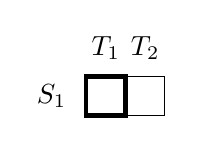
\begin{tikzpicture}[scale=0.5]
  \draw[step=1cm,] (0,0) grid (2,1);
  %\fill[black!20](0,0) rectangle +(1,1);
  \draw[black, ultra thick](0,0) rectangle +(1,1);
\node[anchor=north] at (0.5,2.25) {$T_1$};
\node[anchor=north] at (1.5,2.25) {$T_2$};
\node[anchor=west] at (-1.5,0.5) {$S_1$};
\end{tikzpicture}
& 
\begin{tikzpicture}[scale=0.5]
  \draw[step=1cm,] (0,0) grid (2,1);

(1,0) rectangle +(1,1);
\draw[pattern={north west lines},pattern color=red]
(1,0) rectangle +(1,1);
\draw[pattern={horizontal lines},pattern color=blue](0,0) rectangle (1,1);
\node[anchor=north] at (0.5,2.25) {$T_1$};
\node[anchor=north] at (1.5,2.25) {$T_2$};
\node[anchor=west] at (-1.5,0.5) {$S_1$};
\end{tikzpicture} 
& 
\begin{tikzpicture}[scale=0.5]
  \draw[step=1cm,] (0,0) grid (2,1);
\draw[pattern={north west lines},pattern color=red](0,0) rectangle (1,1);
\draw[pattern={horizontal lines},pattern color=blue](1,0) rectangle +(1,1);
\node[anchor=north] at (0.5,2.25) {$T_1$};
\node[anchor=north] at (1.5,2.25) {$T_2$};
\node[anchor=west] at (-1.5,0.5) {$S_1$};
\end{tikzpicture}\\
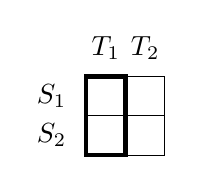
\begin{tikzpicture}[scale=0.5]

%\draw[pattern={north west lines},pattern color=blue](0,0) rectangle +(1,2);
\draw[black, ultra thick](0,0) rectangle +(1,2);
%\draw[pattern={horizontal lines},pattern color=red](1,0) rectangle (2,2);
%\draw[pattern={horizontal lines},pattern color=blue](1,0) rectangle (2,2);
  \draw[step=1cm,] (0,0) grid (2,2);

\node[anchor=north] at (0.5,3.25) {$T_1$};
\node[anchor=north] at (1.5,3.25) {$T_2$};
\node[anchor=west] at (-1.5,1.5) {$S_1$};
\node[anchor=west] at (-1.5,0.5) {$S_2$};
\end{tikzpicture} & \begin{tikzpicture}[scale=0.5]

(0,1) rectangle +(1,1);
\draw[pattern={horizontal lines},pattern color=blue]
(0,1) rectangle +(1,1);
;
\draw[pattern={north west lines},pattern color=red](1,0) rectangle (2,2);
  \draw[step=1cm,] (0,0) grid (2,2);

\node[anchor=north] at (0.5,3.25) {$T_1$};
\node[anchor=north] at (1.5,3.25) {$T_2$};
\node[anchor=west] at (-1.5,1.5) {$S_1$};
\node[anchor=west] at (-1.5,0.5) {$S_2$};
\end{tikzpicture} &
\begin{tikzpicture}[scale=0.5]
(0,0) rectangle +(1,2);
\draw[pattern={north west lines},pattern color=red]
(0,0) rectangle +(1,2);
\draw[pattern={horizontal lines},pattern color=blue](1,1) rectangle +(1,1);
  \draw[step=1cm,] (0,0) grid (2,2);

\node[anchor=north] at (0.5,3.25) {$T_1$};
\node[anchor=north] at (1.5,3.25) {$T_2$};
\node[anchor=west] at (-1.5,1.5) {$S_1$};
\node[anchor=west] at (-1.5,0.5) {$S_2$};
\end{tikzpicture}\\
(a)&(b)&(c)\\

    \end{tabular}
    \end{center}
        \caption{We illustrate the partition for both $\boldsymbol{d}=(1,2)$ and $\boldsymbol{d}=(2,2)$. The set of items $S_1$ can be divided into $T_1$ and $T_2$. If agent $S$ values bundle $T_1 \cap S_1$ (represented with a thick line in (a)) more than $\frac{v_S(S_1)}{2}$ then allocation (b) has the desired properties (the blue bundle for agent $S$ and the red bundle for agent $T$). If this is not the case, then due to the subadditivity, the same holds for agent $S$ and bundle $T_2 \cap S_1$; then (b) has the desired properties.} 
    \label{fig:2agentsRed}
\end{figure}
\end{center}
We also provide a useful restatement of Lemma~\ref{Lemma:2agents} to be used as a reduction tool in the proofs with more agents.
\begin{corollary}
\label{Cor:cut-and-choose}
    Consider a fair division instance of two agents with subadditive valuations and a set of $M$ items, where one agent values $M$ at least $1$, and there exists a partition into two bundles where the other agent values each at least $1/2$. Then, there exists an allocation that guarantees at least $1/2$ value to each agent.
\end{corollary}



\subsection{Three Agents}
\label{sec:3Subadd}
In this section we show that there exists a $1/2$-MMS allocation for the case of three agents. Again, we first show a stronger statement (Lemma~\ref{Lemma:threehalfs}) and obtain the main result as a corollary (Corollary~\ref{cor:3agents}). 

\begin{lemma} [Three agents]
\label{Lemma:threehalfs}
    An $1/2$-MMS$(3,2,2)$ allocation exists for three agents with subadditive valuation functions.
\end{lemma}
\begin{proof}
We denote by $S,T,Q$ the three agents and by $S_j,T_j,Q_j$ their $j$-th MMS bundle, respectively. 

The proof relies on the existence of $(1/2,1)$-MMS$(1,2)$ in the instance with two agents; we show that we can identify a valuable subset $A_T$ (with value at least $1/2$) to allocate to agent $T$, such that we can extend the allocation applying Corollary \ref{Cor:cut-and-choose} for agents $S$ and $Q$ and for the remaining items $M\setminus A_T$. In particular, agent $Q$ will have value at least $1$ for $M\setminus A_T$, while agent $S$ will be able to partition it into two bundles with value at least $1/2$ each. To achieve this we will use two cuts sequentially, first to agent $S$ and then (based on the response of $S$) to agent $T$  (we refer the reader to Figure~\ref{fig:3agents} (a) for an illustration of the proof).
    
{\bf First cut.} Consider the cut $C=T_2$ that we offer to $S$ and let $S_1^*,S_2^* \in \mathcal{X}_{S}^*(C)$ be two bundles in the maximum desired half (by Observation~\ref{obs:Cut_noOfDesiredSets} there exist at least two such bundles). The cut is ``symmetric'' for $T$ in a sense that both $C=T_2$ and $M\setminus C=T_1$ contain the {\em same number of $T$'s MMS bundles}; so it is without loss of generality to assume that $\mathcal{X}^*_S(C)=\mathcal{X}_S(C)$ (in Figure~\ref{fig:3agents} (a) $S_1^* \subseteq S_1,S_2^* \subseteq S_2$ are represented with blue color).

{\bf Second cut.} We next offer $C=Q_1$ to $T$ and let  $T_1^* \in \mathcal{X}_T^*(C)$ be the bundle in the maximum desired half. The cut is ``symmetric'' for $Q$, so again without loss of generality assume that $\mathcal{X}_T^*(C)=\mathcal{X}_T(C)$ (in Figure~\ref{fig:3agents} (b) $T_1^* \subseteq T_1$ is represented with red color).

    
{\bf Apply Corollary \ref{Cor:cut-and-choose}.} Overall, $v_T(T^*_1)\geq 1/2$ and $T^*_1$ will be allocated to $T$. Then, for $M'=M\setminus T^*_1$, it holds that $v_Q(M')\geq v_Q(Q_2) \geq 1$, and $S_1^*,S_2^*\subseteq M'$, for both of which $S$ has value at least $1/2$. So the lemma follows by using Corollary \ref{Cor:cut-and-choose} on $M'$ for agents $Q$ and $S$. (in Figure~\ref{fig:3agents} (c) $S_1^* \subseteq S_1,S_1^* \subseteq S_2$ are represented with blue color and $Q_2$ with green).
\end{proof}
\begin{center}

\begin{figure}
\begin{center}

\begin{tabular}{ccc}

\small{
\begin{tikzpicture}[scale=0.45]
\draw[yslant=0.5,xslant=-1,black, ultra thick](3,3) (5,1) rectangle +(-2,-1);  
\draw[yslant=0.5,black, ultra thick](3,-3) rectangle +(2,3);    \draw[yslant=-0.5,black, ultra thick](3,3) rectangle +(-1,-3); 
\draw[yslant=0.5,xslant=-1,pattern={horizontal lines},pattern color=blue] (5,1) rectangle +(-2,-1);  
\draw[yslant=0.5,pattern={horizontal lines},pattern color=blue](3,-2) rectangle +(2,2);    \draw[yslant=-0.5,pattern={horizontal lines},pattern color=blue](3,3) rectangle +(-1,-2);     

    \draw[yslant=-0.5] (1,0) grid (3,3);
  \draw[yslant=0.5] (3,-3) grid (5,0);
  \draw[yslant=0.5,xslant=-1] (3,0) grid (5,2);
\node[anchor=south west] at (-0.2,1.5,0) {$S_1$};
\node[anchor=south west] at (-0.2,0.5,0) {$S_2$};
\node[anchor=south west] at (-0.2,-0.5,0) {$S_3$};
\node[anchor=north west] at (0.45,3.7,0) {$Q_1$};
\node[anchor=north west] at (1.5,4.3,0) {$Q_2$};
\node[anchor=north west] at (0.5,-0.8,0) {$T_1$};
\node[anchor=north west] at (1.5,-1.3,0) {$T_2$};
\end{tikzpicture}} &
\small{
\begin{tikzpicture}[scale=0.45]
  
    \draw[yslant=0.5,xslant=-1,color=black,ultra thick] (4,2) rectangle +(-1,-2);
    %\fill[yslant=0.5,xslant=-1,color=black!20](4,2) rectangle +(-1,-2); 
    \draw[yslant=0.5,color=black,ultra thick] (3,-3) rectangle +(1,3);
    %\fill[yslant=0.5,color=black!20](3,-3) rectangle +(1,3);

    \draw[yslant=-0.5,color=black,ultra thick](3,3) rectangle +(-2,-3);
    %\fill[yslant=-0.5,color=black!20](3,3) rectangle +(-2,-3);
    
    \draw[yslant=0.5,xslant=-1,pattern={north west lines},pattern color=red](4,2) rectangle +(-1,-1);
\draw[yslant=-0.5,pattern={north west lines},pattern color=red](2,3) rectangle +(-1,-3);
  \draw[yslant=-0.5] (1,0) grid (3,3);
  \draw[yslant=0.5] (3,-3) grid (5,0);
  \draw[yslant=0.5,xslant=-1] (3,0) grid (5,2);
\node[anchor=south west] at (-0.2,1.5,0) {$S_1$};
\node[anchor=south west] at (-0.2,0.5,0) {$S_2$};
\node[anchor=south west] at (-0.2,-0.5,0) {$S_3$};
\node[anchor=north west] at (0.45,3.7,0) {$Q_1$};
\node[anchor=north west] at (1.5,4.3,0) {$Q_2$};
\node[anchor=north west] at (0.5,-0.8,0) {$T_1$};
\node[anchor=north west] at (1.5,-1.3,0) {$T_2$};
\end{tikzpicture}} &
\small{
\begin{tikzpicture}[scale=0.45]
 \draw[yslant=0.5,xslant=-1,pattern={north west lines},pattern color=red](4,2) rectangle +(-1,-1);
\draw[yslant=-0.5,pattern={north west lines},pattern color=red](2,3) rectangle +(-1,-3);
\draw[yslant=0.5,xslant=-1,pattern={crosshatch dots},pattern color=green]  (5,2) rectangle +(-1,-2);
    \draw[yslant=0.5,pattern={crosshatch dots},pattern color=green]  (4,-3) rectangle +(1,3);

    \draw[yslant=0.5,xslant=-1,pattern={horizontal lines},pattern color=blue] (5,1) rectangle +(-2,-1);
    \draw[yslant=0.5,pattern={horizontal lines},pattern color=blue](3,-2) rectangle +(2,2);
    \draw[yslant=-0.5,pattern={horizontal lines},pattern color=blue](3,3) rectangle (2,1);
  \draw[yslant=-0.5] (1,0) grid (3,3);
  \draw[yslant=0.5] (3,-3) grid (5,0);
  \draw[yslant=0.5,xslant=-1] (3,0) grid (5,2);
\node[anchor=south west] at (-0.2,1.5,0) {$S_1$};
\node[anchor=south west] at (-0.2,0.5,0) {$S_2$};
\node[anchor=south west] at (-0.2,-0.5,0) {$S_3$};
\node[anchor=north west] at (0.45,3.7,0) {$Q_1$};
\node[anchor=north west] at (1.5,4.3,0) {$Q_2$};
\node[anchor=north west] at (0.5,-0.8,0) {$T_1$};
\node[anchor=north west] at (1.5,-1.3,0) {$T_2$};
\end{tikzpicture}}\\
(a) & (b) & (c) \\
$S_1^*,S_2^* \in \mathcal{X}_S^*(T_2)$ &  $T_1^* \in \mathcal{X}^*_T(Q_1)$ & Apply Corollary \ref{Cor:cut-and-choose}\\
\end{tabular}
    
\end{center}
\caption{We use blue, red, and green to denote the bundles from which we will allocate to agents $S,T$ and $Q$, respectively. The thickened lines illustrate the first and second cuts, while (c) demonstrates the application of Corollary 2.
}
\label{fig:3agents}
\end{figure} 
\end{center}
As a corollary of Lemma~\ref{Lemma:threehalfs}, a $1/2$-MMS allocation always exists for three agents (by Observation~\ref{obs:simpleReduction}); this bound is also tight \cite{GhodsiHSSY22}. 
\begin{corollary}
\label{cor:3agents}
    A $1/2$-MMS allocation exists for three agents with subadditive valuation functions. 
\end{corollary}


\subsection{Four Agents}
In this section we show the existence of $1/2$-MMS allocation for the case of four agents, our main technical result. We are also able to show a stronger statement (Lemma~\ref{Lemma:4agents}) and obtain the main result as a corollary (Corollary~\ref{cor:4agents}). 

\label{sec:4Subadd}

\begin{lemma} [Four agents]
\label{Lemma:4agents}
    A $1/2$-MMS$(3,3,4,4)$ allocation exists for four agents with subadditive valuation functions.
\end{lemma}
\begin{proof}
    We denote by $S,T,Q,R$ the four agents and by $S_j,T_j,Q_j,R_j$ their $j$-th MMS bundle, respectively. 
    
    We progressively identify four candidate allocations in total, and we show that one of those should be a $1/2$-MMS$(3,3,4,4)$ allocation. 

    In a nutshell, the protocol works as follows. By offering carefully chosen cuts to agents $S,T,Q$ we are able to find partial allocations for two of those agents (in the first round these are $S$ and $T$), that have high enough value (higher than $1/2$), in a way that always preserves one MMS bundle of agent $R$ {\em intact}, let it be $R_4$. If the third agent (this is $Q$ in the first round) values higher than $1/2$ two of her bundles (on the remaining items) then we can apply Corollary~\ref{Cor:cut-and-choose} on $Q$ and $R$ and for the remaining items, and we can claim a $1/2$-MMS$(3,3,4,4)$ allocation. If this is not the case, then the third agent must value at least two of the intersections of her bundles with the partial allocation of the other two agents with value higher than $1/2$. In the next round we will tentatively allocate to the third agent one of these sets. We will also keep one of the other two agents and offer her a subset of high value {\em from a different bundle} (the notion of maximum desired half is useful to achieve this last property). We proceed in a similar manner by querying the remaining agent investigating again whether Corollary~\ref{Cor:cut-and-choose} can be employed. The key is that in every round that the third agent does not satisfy the conditions of Corollary~\ref{Cor:cut-and-choose} we are able to build a more structured partial allocation, which in the final step provides an allocation of $M\setminus R_4$ to agents $S,T$ and $Q$, that they value by at least $1/2$. Then $R_4$ can be allocated to agent $R$ and the allocation is $1/2$-MMS$(3,3,4,4)$.
    
\begin{center}

\begin{figure}[t]
\begin{center}

    \begin{tabular}{cc}
\small{
\begin{tikzpicture}[scale=0.425]
\draw[yslant=0.5,ultra thick, black](4,-3) rectangle +(4,1);     
\draw[yslant=-0.5,ultra thick, black](4,2) rectangle +(-3,-1); 
\draw[yslant=-0.5,pattern={north west lines},pattern color=red](4,3) rectangle +(-1,-1);
\draw[yslant=-0.5,pattern={north west lines},pattern color=red](4,1) rectangle +(-1,-1);
\draw[yslant=0.5,xslant=-1,pattern={north west lines},pattern color=red](7,0) rectangle +(-4,-1); 
\draw[yslant=0.5,pattern={north west lines},pattern color=red](4,-2) rectangle +(4,1);   
\draw[yslant=0.5,pattern={north west lines},pattern color=red](4,-4) rectangle +(4,1);   
%\draw[yslant=0.5,xslant=-1,pattern={horizontal lines},pattern color=blue](7,2) rectangle +(-4,-3);  
\draw[yslant=0.5,pattern={horizontal lines},pattern color=blue](4,-3) rectangle +(4,1);     
\draw[yslant=-0.5,pattern={horizontal lines},pattern color=blue](4,2) rectangle +(-3,-1);     
  \draw[yslant=-0.5] (1,0) grid (4,3);
  \draw[yslant=0.5] (4,-4) grid (8,-1);
  \draw[yslant=0.5,xslant=-1] (3,-1) grid (7,2);
\node[anchor=south west] at (-0.25,1.5,0) {$S_1$};
\node[anchor=south west] at (-0.25,0.5,0) {$S_2$};
\node[anchor=south west] at (-0.25,-0.5,0) {$S_3$};
\node[anchor=north west] at (0.5,3.8,0) {$Q_1$};
\node[anchor=north west] at (1.5,4.3,0) {$Q_2$};
\node[anchor=north west] at (2.5,4.8,0) {$Q_3$};
\node[anchor=north west] at (3.5,5.3,0) {$Q_4$};
\node[anchor=north west] at (0.4,-0.8,0) {$T_3$};
\node[anchor=north west] at (1.4,-1.3,0) {$T_2$};
\node[anchor=north west] at (2.4,-1.8,0) {$T_1$};
\node[anchor=north] at (7,5,0) {$R_1$};
\end{tikzpicture}}
&
\small{
\begin{tikzpicture}[scale=0.425]
\draw[yslant=0.5,ultra thick, black](4,-3) rectangle +(4,1);     
\draw[yslant=-0.5,ultra thick, black](4,2) rectangle +(-3,-1); 
\draw[yslant=-0.5,pattern={north west lines},pattern color=red](4,3) rectangle +(-1,-1);
\draw[yslant=-0.5,pattern={north west lines},pattern color=red](4,1) rectangle +(-1,-1);
\draw[yslant=0.5,xslant=-1,pattern={north west lines},pattern color=red](7,0) rectangle +(-4,-1); 
\draw[yslant=0.5,pattern={north west lines},pattern color=red](4,-2) rectangle +(4,1);   
\draw[yslant=0.5,pattern={north west lines},pattern color=red](4,-4) rectangle +(4,1);   
%\draw[yslant=0.5,xslant=-1,pattern={horizontal lines},pattern color=blue](7,2) rectangle +(-4,-3);  
\draw[yslant=0.5,pattern={horizontal lines},pattern color=blue](4,-3) rectangle +(4,1);     
\draw[yslant=-0.5,pattern={horizontal lines},pattern color=blue](4,2) rectangle +(-3,-1);      
  \draw[yslant=-0.5] (1,0) grid (4,3);
  \draw[yslant=0.5] (4,-4) grid (8,-1);
  \draw[yslant=0.5,xslant=-1] (3,-1) grid (7,2);
\node[anchor=south west] at (-0.25,1.5,0) {$S_1$};
\node[anchor=south west] at (-0.25,0.5,0) {$S_2$};
\node[anchor=south west] at (-0.25,-0.5,0) {$S_3$};
\node[anchor=north west] at (0.5,3.8,0) {$Q_1$};
\node[anchor=north west] at (1.5,4.3,0) {$Q_2$};
\node[anchor=north west] at (2.5,4.8,0) {$Q_3$};
\node[anchor=north west] at (3.5,5.3,0) {$Q_4$};
\node[anchor=north west] at (0.4,-0.8,0) {$T_3$};
\node[anchor=north west] at (1.4,-1.3,0) {$T_2$};
\node[anchor=north west] at (2.4,-1.8,0) {$T_1$};
\node[anchor=north] at (7,5,0) {$R_2$};
\end{tikzpicture}}\\
\small{
\begin{tikzpicture}[scale=0.425]
\draw[yslant=-0.5,pattern={north west lines},pattern color=red](4,3) rectangle +(-1,-3);
\draw[yslant=0.5,xslant=-1,pattern={north west lines},pattern color=red](7,0) rectangle +(-4,-1); 
\draw[yslant=0.5,pattern={north west lines},pattern color=red](4,-4) rectangle +(4,3);    
  \draw[yslant=-0.5] (1,0) grid (4,3);
  \draw[yslant=0.5] (4,-4) grid (8,-1);
  \draw[yslant=0.5,xslant=-1] (3,-1) grid (7,2);
\node[anchor=south west] at (-0.25,1.5,0) {$S_1$};
\node[anchor=south west] at (-0.25,0.5,0) {$S_2$};
\node[anchor=south west] at (-0.25,-0.5,0) {$S_3$};
\node[anchor=north west] at (0.5,3.8,0) {$Q_1$};
\node[anchor=north west] at (1.5,4.3,0) {$Q_2$};
\node[anchor=north west] at (2.5,4.8,0) {$Q_3$};
\node[anchor=north west] at (3.5,5.3,0) {$Q_4$};
\node[anchor=north west] at (0.4,-0.8,0) {$T_3$};
\node[anchor=north west] at (1.4,-1.3,0) {$T_2$};
\node[anchor=north west] at (2.4,-1.8,0) {$T_1$};
\node[anchor=north] at (7,5,0) {$R_3$};
\end{tikzpicture}}
&

\small{
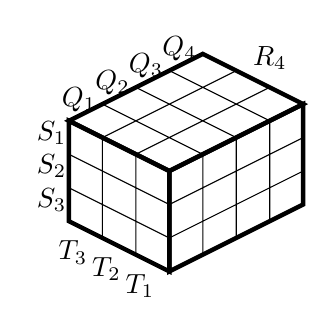
\begin{tikzpicture}[scale=0.425]
\draw[yslant=0.5,ultra thick, black](4,-4) rectangle +(4,3);     
\draw[yslant=-0.5,ultra thick, black](4,3) rectangle +(-3,-3); 
\draw[yslant=0.5,xslant=-1,ultra thick, black](7,2) rectangle +(-4,-3);    
  \draw[yslant=-0.5] (1,0) grid (4,3);
  \draw[yslant=0.5] (4,-4) grid (8,-1);
  \draw[yslant=0.5,xslant=-1] (3,-1) grid (7,2);
\node[anchor=south west] at (-0.25,1.5,0) {$S_1$};
\node[anchor=south west] at (-0.25,0.5,0) {$S_2$};
\node[anchor=south west] at (-0.25,-0.5,0) {$S_3$};
\node[anchor=north west] at (0.5,3.8,0) {$Q_1$};
\node[anchor=north west] at (1.5,4.3,0) {$Q_2$};
\node[anchor=north west] at (2.5,4.8,0) {$Q_3$};
\node[anchor=north west] at (3.5,5.3,0) {$Q_4$};
\node[anchor=north west] at (0.4,-0.8,0) {$T_3$};
\node[anchor=north west] at (1.4,-1.3,0) {$T_2$};
\node[anchor=north west] at (2.4,-1.8,0) {$T_1$};
\node[anchor=north] at (7,5,0) {$R_4$};
\end{tikzpicture}}\\
\end{tabular}
    
\end{center}
\caption{The first candidate allocation $A=(S_2^*,T_1^*)$ for four agents and $\boldsymbol{d}=(3,3,4,4)$. We use blue to denote $S_2^* \subseteq S_2$ and red to denote $T_1^* \subseteq T_1$. We use a thick line to illustrate the cut $C=\{S^*_2 \cup R_4\}$. The allocation is valid and none of the bundles intersects with $R_4$. The cuts are symmetric, i.e. if we had $\mathcal{X}_S^*(C) =\mathcal{X}_S^*(M\setminus C)$ for cut $C=\{R_1 \cup R_2\}$ or/and $\mathcal{X}_T^*(C)=\mathcal{X}_T(C)$ for the corresponding cut $C$, we could construct the same allocation by renaming the bundles.}
\label{fig:4agents1}
\end{figure}
\end{center}



    
  
    
    \noindent{\bf Building the first candidate allocation}. We first consider agent $S$ (an agent with $3$ MMS bundles) and cut her MMS bundles by offering the cut $C=R_1 \cup R_2$. By Observation~\ref{obs:Cut_noOfDesiredSets} there are at least two bundles in the set $\mathcal{X}_{S}^*(C)$; let those be $S_1^*,S_2^* \in \mathcal{X}_{S}^*(C)$. We note that $S_1^*,S_2^*$ intersect with exactly two MMS bundles of $R$, so w.l.o.g. assume that those are $R_1,R_2$, i.e., assume that $\mathcal{X}_{S}^*(C)=\mathcal{X}_{S}(C)$. Therefore
     \begin{equation}
        \label{eq:4agentsCond0}
        S_j^*\cap R_3 = \emptyset \mbox{ and } S_j^*\cap R_4 = \emptyset, \mbox{ for } j \in \{1,2\}\,.
    \end{equation}
    

    Next, we offer a cut to agent $T$ in a way that a) ensures that a {\em whole} MMS bundle of agent $R$ remains intact and b) one of $S_1^*, S_2^*$ does not intersect with the Maximum Desired Half of $T$. A cut that serves this purpose is $C=S_2^* \cup R_4$. Now each of the sets $C$ and $M\setminus C$ intersects with exactly one of $S^*_1, S^*_2$ and with exactly one of $R_3, R_4$ which are the remaining whole bundles of $R$. W.l.o.g. assume that $\mathcal{X}_{T}^*(C)=\mathcal{X}_{T}(M \setminus C)$.\footnote{Even if it is w.l.o.g., we consider $\mathcal{X}_{T}^*(C)=\mathcal{X}_{T}(M \setminus C)$ that includes $S_3$ to avoid any confusion of the steps needed, because the case of $\mathcal{X}_{T}^*(C)=\mathcal{X}_{T}(C)$ is simpler and can be handled the same way.} 
    By Observation~\ref{obs:Cut_noOfDesiredSets} there are at least two bundles in the set $\mathcal{X}_{T}^*(C)$, let those be $T_1^*,T_2^* \in \mathcal{X}_{T}^*(C)$. Then, it holds that 
    \begin{equation}
    \label{eq:4agentsCond1}
        T_j^*\cap R_4 = \emptyset \mbox{ and } T_j^*\cap S_2^* = \emptyset, \mbox{ for } j \in \{1,2\}\,.
    \end{equation}
    
    {\bf First candidate allocation.} Consider the following partial allocation for $S$ and $T$: $A= (S^*_2,T^*_1)$ (see Figure \ref{fig:4agents1} for an illustration). By construction, both $S$ and $T$ value their allocated bundles by at least $1/2$. If there exist at least two MMS bundles of $Q$ that she values with at least $1/2$ {\em after the removal of $S^*_2\cup T^*_1$}, then the conditions of Corollary~\ref{Cor:cut-and-choose} are satisfied for $Q$ and $R$ for the remaining items (recall that $R$ values the remaining items by at least $1$ since they contain $R_4$). Hence by  employing Corollary~\ref{Cor:cut-and-choose} we can find an allocation of $M\setminus (S^*_2\cup T^*_1)$ to $Q$ and $R$ where they both value their bundles with at least $1/2$, and we are done.   
        
    So, suppose that this is not the case. Then there must be at least three MMS bundles of $Q$, let them be $Q_1,Q_2,Q_3$, such that $v_Q(Q_j\cap(S^*_2\cup T^*_1))\geq 1/2$ for $j\in\{1, 2, 3\}$. In other words, if we consider the cut $C=S^*_2\cup T^*_1$ for agent $Q$, then it is guaranteed that $Q_1^*,Q^*_2,Q^*_3 \in \mathcal{X}_{Q}(C)$. Since $Q_j^*\subseteq S^*_2\cup T^*_1$, for all $j \in \{1,2,3\}$ and also by \eqref{eq:4agentsCond0} and \eqref{eq:4agentsCond1} we conclude that
    \begin{equation}
        \label{eq:4agentsCond2}
        Q_j^* \cap T^*_2 = \emptyset \mbox{ and } Q_j^* \cap R_4= \emptyset , \mbox{ for } j \in \{1,2,3\}\,.
    \end{equation}


    \begin{figure}[h] 
\begin{center}
    \begin{tabular}{cc}
\small{
\begin{tikzpicture}[scale=0.425]
\draw[yslant=-0.5,ultra thick, black](4,3) rectangle +(-1,-3);
\draw[yslant=0.5,xslant=-1,ultra thick, black](7,0) rectangle +(-4,-1); 
\draw[yslant=0.5,ultra thick, black](4,-4) rectangle +(4,3);   
       
\draw[yslant=-0.5,ultra thick, black](3,2) rectangle +(-2,-1);
\draw[yslant=-0.5,ultra thick, white](3,2) rectangle +(0,-1);
\draw[yslant=0.5,pattern={crosshatch dots},pattern color=green] (4,-4) rectangle +(1,3);
\draw[yslant=-0.5,pattern={crosshatch dots},pattern color=green](4,3) rectangle +(-1,-3);
\draw[yslant=-0.5,pattern={crosshatch dots},pattern color=green](3,2) rectangle +(-2,-1);
\draw[yslant=-0.5,pattern={north west lines},pattern color=red](3,3) rectangle +(-1,-1);
\draw[yslant=-0.5,pattern={north west lines},pattern color=red](3,1) rectangle +(-1,-1);
\draw[yslant=0.5,xslant=-1,pattern={north west lines},pattern color=red](7,1) rectangle +(-4,-1); 
\draw[yslant=0.5,xslant=-1,pattern={crosshatch dots},pattern color=green](4,0) rectangle +(-1,-1);     
  \draw[yslant=-0.5] (1,0) grid (4,3);
  \draw[yslant=0.5] (4,-4) grid (8,-1);
  \draw[yslant=0.5,xslant=-1] (3,-1) grid (7,2);
\node[anchor=south west] at (-0.25,1.5,0) {$S_1$};
\node[anchor=south west] at (-0.25,0.5,0) {$S_2$};
\node[anchor=south west] at (-0.25,-0.5,0) {$S_3$};
\node[anchor=north west] at (0.5,3.8,0) {$Q_1$};
\node[anchor=north west] at (1.5,4.3,0) {$Q_2$};
\node[anchor=north west] at (2.5,4.8,0) {$Q_3$};
\node[anchor=north west] at (3.5,5.3,0) {$Q_4$};
\node[anchor=north west] at (0.4,-0.8,0) {$T_3$};
\node[anchor=north west] at (1.4,-1.3,0) {$T_2$};
\node[anchor=north west] at (2.4,-1.8,0) {$T_1$};
\node[anchor=north] at (7,5,0) {$R_1$};
\end{tikzpicture}}
&
\small{
\begin{tikzpicture}[scale=0.425]
\draw[yslant=-0.5,ultra thick, black](4,3) rectangle +(-1,-3);
\draw[yslant=0.5,xslant=-1,ultra thick, black](7,0) rectangle +(-4,-1); 
\draw[yslant=0.5,ultra thick, black](4,-4) rectangle +(4,3);   
       
\draw[yslant=-0.5,ultra thick, black](3,2) rectangle +(-2,-1);
\draw[yslant=-0.5,ultra thick, white](3,2) rectangle +(0,-1);
\draw[yslant=0.5,pattern={crosshatch dots},pattern color=green] (4,-4) rectangle +(1,3);
\draw[yslant=-0.5,pattern={crosshatch dots},pattern color=green](4,3) rectangle +(-1,-3);
\draw[yslant=-0.5,pattern={crosshatch dots},pattern color=green](3,2) rectangle +(-2,-1);
\draw[yslant=-0.5,pattern={north west lines},pattern color=red](3,3) rectangle +(-1,-1);
\draw[yslant=-0.5,pattern={north west lines},pattern color=red](3,1) rectangle +(-1,-1);
\draw[yslant=0.5,xslant=-1,pattern={north west lines},pattern color=red](7,1) rectangle +(-4,-1); 
\draw[yslant=0.5,xslant=-1,pattern={crosshatch dots},pattern color=green](4,0) rectangle +(-1,-1);    
  \draw[yslant=-0.5] (1,0) grid (4,3);
  \draw[yslant=0.5] (4,-4) grid (8,-1);
  \draw[yslant=0.5,xslant=-1] (3,-1) grid (7,2);
\node[anchor=south west] at (-0.25,1.5,0) {$S_1$};
\node[anchor=south west] at (-0.25,0.5,0) {$S_2$};
\node[anchor=south west] at (-0.25,-0.5,0) {$S_3$};
\node[anchor=north west] at (0.5,3.8,0) {$Q_1$};
\node[anchor=north west] at (1.5,4.3,0) {$Q_2$};
\node[anchor=north west] at (2.5,4.8,0) {$Q_3$};
\node[anchor=north west] at (3.5,5.3,0) {$Q_4$};
\node[anchor=north west] at (0.4,-0.8,0) {$T_3$};
\node[anchor=north west] at (1.4,-1.3,0) {$T_2$};
\node[anchor=north west] at (2.4,-1.8,0) {$T_1$};
\node[anchor=north] at (7,5,0) {$R_2$};
\end{tikzpicture}}\\
\small{
\begin{tikzpicture}[scale=0.425]
\draw[yslant=-0.5,ultra thick, black](4,3) rectangle +(-1,-3);
\draw[yslant=0.5,xslant=-1,ultra thick, black](7,0) rectangle +(-4,-1); 
\draw[yslant=0.5,ultra thick, black](4,-4) rectangle +(4,3);   
       
\draw[yslant=-0.5,pattern={north west lines},pattern color=red](3,3) rectangle +(-1,-3);
\draw[yslant=0.5,xslant=-1,pattern={north west lines},pattern color=red](7,1) rectangle +(-4,-1); 
\draw[yslant=-0.5,pattern={crosshatch dots},pattern color=green](4,3) rectangle +(-1,-3);
\draw[yslant=0.5,xslant=-1,pattern={crosshatch dots},pattern color=green](4,0) rectangle +(-1,-1); 
\draw[yslant=0.5,pattern={crosshatch dots},pattern color=green](4,-4) rectangle +(1,3);    
  \draw[yslant=-0.5] (1,0) grid (4,3);
  \draw[yslant=0.5] (4,-4) grid (8,-1);
  \draw[yslant=0.5,xslant=-1] (3,-1) grid (7,2);
\node[anchor=south west] at (-0.25,1.5,0) {$S_1$};
\node[anchor=south west] at (-0.25,0.5,0) {$S_2$};
\node[anchor=south west] at (-0.25,-0.5,0) {$S_3$};
\node[anchor=north west] at (0.5,3.8,0) {$Q_1$};
\node[anchor=north west] at (1.5,4.3,0) {$Q_2$};
\node[anchor=north west] at (2.5,4.8,0) {$Q_3$};
\node[anchor=north west] at (3.5,5.3,0) {$Q_4$};
\node[anchor=north west] at (0.4,-0.8,0) {$T_3$};
\node[anchor=north west] at (1.4,-1.3,0) {$T_2$};
\node[anchor=north west] at (2.4,-1.8,0) {$T_1$};
\node[anchor=north] at (7,5,0) {$R_3$};
\end{tikzpicture}}
&

\small{
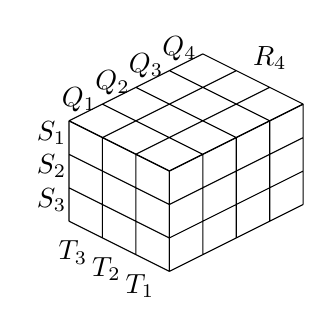
\begin{tikzpicture}[scale=0.425]

    
  \draw[yslant=-0.5] (1,0) grid (4,3);
  \draw[yslant=0.5] (4,-4) grid (8,-1);
  \draw[yslant=0.5,xslant=-1] (3,-1) grid (7,2);
\node[anchor=south west] at (-0.25,1.5,0) {$S_1$};
\node[anchor=south west] at (-0.25,0.5,0) {$S_2$};
\node[anchor=south west] at (-0.25,-0.5,0) {$S_3$};
\node[anchor=north west] at (0.5,3.8,0) {$Q_1$};
\node[anchor=north west] at (1.5,4.3,0) {$Q_2$};
\node[anchor=north west] at (2.5,4.8,0) {$Q_3$};
\node[anchor=north west] at (3.5,5.3,0) {$Q_4$};
\node[anchor=north west] at (0.4,-0.8,0) {$T_3$};
\node[anchor=north west] at (1.4,-1.3,0) {$T_2$};
\node[anchor=north west] at (2.4,-1.8,0) {$T_1$};
\node[anchor=north] at (7,5,0) {$R_4$};
\end{tikzpicture}}\\
\end{tabular}
    
\end{center}
\caption{The second candidate allocation $A'=(T_2^*,Q_1^*)$. We use red for bundle $T_2^* \subseteq T_2$ and green for $Q_1^*\subseteq Q_1$. The cut $C=\{T_1^* \cup S_2^*\}$ is shown with a thick line. We try to apply Corollary \ref{cor:2agents} for agents $S$ and $R$ and the set of items $M \setminus (T_2^*\cup Q_1^*)$. We could construct the same allocation for any $3$ bundles $Q_i^*$ by renaming the bundles.}
\label{fig:4agents2}
\end{figure}

    {\bf Second candidate allocation.} Next, we consider the partial allocation $A'= (T^*_2,Q^*_1)$ for agents $T$ and $Q$ which by (\ref{eq:4agentsCond2}) is valid and both $v_T(T^*_2), v_Q(Q_1^*)$ are higher than $1/2$ (see Figure \ref{fig:4agents2} for an illustration). If there exist at least two MMS bundles of $S$, that she values with at least $1/2$ {\em after the removal of $T^*_2 \cup Q^*_1$}, then by employing Corollary \ref{Cor:cut-and-choose} we can find an allocation of $M\setminus (T^*_2\cup Q^*_1)$ to $S$ and $R$ where they both value their bundles with at least $1/2$, and we are done.
    
    
    Otherwise, it should be that for the cut $C=T^*_2 \cup Q^*_1$  there are two sets\footnote{We note that it is not necessarily the case that $S'_1\subseteq S_1$ or $S'_2\subseteq S_2$ although this is how it is depicted in the figures for the sake of exposition.} $S_1',S_2' \in \mathcal{X}_{S}(C)$. 
    Since for any $j \in \{1,2\}$, $S_j'\subseteq T^*_2 \cup Q^*_1$, by \eqref{eq:4agentsCond1} and \eqref{eq:4agentsCond2} we conclude
    \begin{equation}
        \label{eq:4agentsCond3}
        S_j' \cap Q^*_2 = \emptyset, S_j' \cap Q^*_3 = \emptyset \mbox{ and } S_j' \cap R_4 = \emptyset, \mbox{ for } j \in \{1,2\}\,.
    \end{equation}
    
    
    {\bf Third candidate allocation.} Consider now the partial allocation $A''= (S'_1,Q^*_2)$ for $S$ and $Q$, which is valid (due to (\ref{eq:4agentsCond3})) and both agents value their allocated bundles by at least $1/2$ (see Figure \ref{fig:4agents3} for an illustration).
    Again, if there exist at least two MMS bundles of $T$, that she values with at least $1/2$ after the removal of $S'_1\cup Q^*_2$, by using Corollary \ref{Cor:cut-and-choose} on $T$ and $R$, we are done (similarly as in the previous cases). 
    
 
  

\begin{figure}[H]
\begin{center}

    \begin{tabular}{cc}
\small{
\begin{tikzpicture}[scale=0.425]
      
 
\draw[yslant=0.5,ultra thick, black] (4,-4) rectangle +(1,3);
\draw[yslant=-0.5,ultra thick, black](4,3) rectangle +(-2,-3);
\draw[yslant=-0.5,ultra thick, black](2,2) rectangle +(-1,-1);
\draw[yslant=-0.5,ultra thick, white](3,1) rectangle +(-1,1);
\draw[yslant=0.5,xslant=-1,ultra thick, black](7,1) rectangle +(-4,-1); 
\draw[yslant=0.5,xslant=-1,ultra thick, black](4,0) rectangle +(-1,-1); 
\draw[yslant=0.5,xslant=-1,ultra thick, white](3,0) rectangle +(1,0); 

\draw[yslant=0.5,pattern={crosshatch dots},pattern color=green] (5,-4) rectangle +(1,3);
\draw[yslant=0.5,xslant=-1,pattern={crosshatch dots},pattern color=green](5,0) rectangle +(-1,-1); 
\draw[yslant=0.5,pattern={horizontal lines},pattern color=blue](4,-2) rectangle +(1,1);    
\draw[yslant=0.5,xslant=-1,pattern={horizontal lines},pattern color=blue](7,1) rectangle +(-4,-1);
\draw[yslant=0.5,xslant=-1,pattern={horizontal lines},pattern color=blue](4,0) rectangle +(-1,-1);
%\draw[yslant=-0.5,pattern={horizontal lines},pattern color=blue](4,2) rectangle +(-3,-1);     
\draw[yslant=-0.5,pattern={horizontal lines},pattern color=blue](4,3) rectangle +(-2,-1);    
  \draw[yslant=-0.5] (1,0) grid (4,3);
  \draw[yslant=0.5] (4,-4) grid (8,-1);
  \draw[yslant=0.5,xslant=-1] (3,-1) grid (7,2);
\node[anchor=south west] at (-0.25,1.5,0) {$S_1$};
\node[anchor=south west] at (-0.25,0.5,0) {$S_2$};
\node[anchor=south west] at (-0.25,-0.5,0) {$S_3$};
\node[anchor=north west] at (0.5,3.8,0) {$Q_1$};
\node[anchor=north west] at (1.5,4.3,0) {$Q_2$};
\node[anchor=north west] at (2.5,4.8,0) {$Q_3$};
\node[anchor=north west] at (3.5,5.3,0) {$Q_4$};
\node[anchor=north west] at (0.4,-0.8,0) {$T_3$};
\node[anchor=north west] at (1.4,-1.3,0) {$T_2$};
\node[anchor=north west] at (2.4,-1.8,0) {$T_1$};
\node[anchor=north] at (7,5,0) {$R_1$};
\end{tikzpicture}}
&
\small{
\begin{tikzpicture}[scale=0.425]

\draw[yslant=0.5,ultra thick, black] (4,-4) rectangle +(1,3);
\draw[yslant=-0.5,ultra thick, black](4,3) rectangle +(-2,-3);
\draw[yslant=-0.5,ultra thick, black](2,2) rectangle +(-1,-1);
\draw[yslant=-0.5,ultra thick, white](3,1) rectangle +(-1,1);
\draw[yslant=0.5,xslant=-1,ultra thick, black](7,1) rectangle +(-4,-1); 
\draw[yslant=0.5,xslant=-1,ultra thick, black](4,0) rectangle +(-1,-1); 
\draw[yslant=0.5,xslant=-1,ultra thick, white](3,0) rectangle +(1,0); 

\draw[yslant=0.5,pattern={crosshatch dots},pattern color=green] (5,-4) rectangle +(1,3);

\draw[yslant=0.5,xslant=-1,pattern={crosshatch dots},pattern color=green](5,0) rectangle +(-1,-1); 
\draw[yslant=0.5,pattern={horizontal lines},pattern color=blue](4,-2) rectangle +(1,1);    
\draw[yslant=0.5,xslant=-1,pattern={horizontal lines},pattern color=blue](7,1) rectangle +(-4,-1);
\draw[yslant=0.5,xslant=-1,pattern={horizontal lines},pattern color=blue](4,0) rectangle +(-1,-1);
%\draw[yslant=-0.5,pattern={horizontal lines},pattern color=blue](4,2) rectangle +(-3,-1);     
\draw[yslant=-0.5,pattern={horizontal lines},pattern color=blue](4,3) rectangle +(-2,-1);  
  \draw[yslant=-0.5] (1,0) grid (4,3);
  \draw[yslant=0.5] (4,-4) grid (8,-1);
  \draw[yslant=0.5,xslant=-1] (3,-1) grid (7,2);
\node[anchor=south west] at (-0.25,1.5,0) {$S_1$};
\node[anchor=south west] at (-0.25,0.5,0) {$S_2$};
\node[anchor=south west] at (-0.25,-0.5,0) {$S_3$};
\node[anchor=north west] at (0.5,3.8,0) {$Q_1$};
\node[anchor=north west] at (1.5,4.3,0) {$Q_2$};
\node[anchor=north west] at (2.5,4.8,0) {$Q_3$};
\node[anchor=north west] at (3.5,5.3,0) {$Q_4$};
\node[anchor=north west] at (0.4,-0.8,0) {$T_3$};
\node[anchor=north west] at (1.4,-1.3,0) {$T_2$};
\node[anchor=north west] at (2.4,-1.8,0) {$T_1$};
\node[anchor=north] at (7,5,0) {$R_2$};
\end{tikzpicture}}\\
\small{
\begin{tikzpicture}[scale=0.425]
\draw[yslant=0.5,ultra thick, black] (4,-4) rectangle +(1,3);
\draw[yslant=-0.5,ultra thick, black](4,3) rectangle +(-2,-3);
\draw[yslant=0.5,xslant=-1,ultra thick, black](7,1) rectangle +(-4,-1); 
\draw[yslant=0.5,xslant=-1,ultra thick, black](4,0) rectangle +(-1,-1); 
\draw[yslant=0.5,xslant=-1,ultra thick, white](3,0) rectangle +(1,0); 

\draw[yslant=0.5,pattern={crosshatch dots},pattern color=green] (5,-4) rectangle +(1,3);

\draw[yslant=0.5,xslant=-1,pattern={crosshatch dots},pattern color=green](5,0) rectangle +(-1,-1); 
\draw[yslant=0.5,pattern={horizontal lines},pattern color=blue](4,-2) rectangle +(1,1);    
\draw[yslant=0.5,xslant=-1,pattern={horizontal lines},pattern color=blue](7,1) rectangle +(-4,-1);
\draw[yslant=0.5,xslant=-1,pattern={horizontal lines},pattern color=blue](4,0) rectangle +(-1,-1);
%\draw[yslant=-0.5,pattern={horizontal lines},pattern color=blue](4,2) rectangle +(-3,-1);     
\draw[yslant=-0.5,pattern={horizontal lines},pattern color=blue](4,3) rectangle +(-2,-1);
  \draw[yslant=-0.5] (1,0) grid (4,3);
  \draw[yslant=0.5] (4,-4) grid (8,-1);
  \draw[yslant=0.5,xslant=-1] (3,-1) grid (7,2);
\node[anchor=south west] at (-0.25,1.5,0) {$S_1$};
\node[anchor=south west] at (-0.25,0.5,0) {$S_2$};
\node[anchor=south west] at (-0.25,-0.5,0) {$S_3$};
\node[anchor=north west] at (0.5,3.8,0) {$Q_1$};
\node[anchor=north west] at (1.5,4.3,0) {$Q_2$};
\node[anchor=north west] at (2.5,4.8,0) {$Q_3$};
\node[anchor=north west] at (3.5,5.3,0) {$Q_4$};
\node[anchor=north west] at (0.4,-0.8,0) {$T_3$};
\node[anchor=north west] at (1.4,-1.3,0) {$T_2$};
\node[anchor=north west] at (2.4,-1.8,0) {$T_1$};
\node[anchor=north] at (7,5,0) {$R_3$};
\end{tikzpicture}}
&

\small{
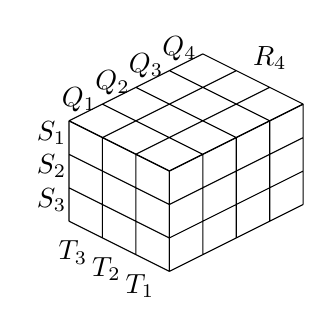
\begin{tikzpicture}[scale=0.425]

    
  \draw[yslant=-0.5] (1,0) grid (4,3);
  \draw[yslant=0.5] (4,-4) grid (8,-1);
  \draw[yslant=0.5,xslant=-1] (3,-1) grid (7,2);
\node[anchor=south west] at (-0.25,1.5,0) {$S_1$};
\node[anchor=south west] at (-0.25,0.5,0) {$S_2$};
\node[anchor=south west] at (-0.25,-0.5,0) {$S_3$};
\node[anchor=north west] at (0.5,3.8,0) {$Q_1$};
\node[anchor=north west] at (1.5,4.3,0) {$Q_2$};
\node[anchor=north west] at (2.5,4.8,0) {$Q_3$};
\node[anchor=north west] at (3.5,5.3,0) {$Q_4$};
\node[anchor=north west] at (0.4,-0.8,0) {$T_3$};
\node[anchor=north west] at (1.4,-1.3,0) {$T_2$};
\node[anchor=north west] at (2.4,-1.8,0) {$T_1$};
\node[anchor=north] at (7,5,0) {$R_4$};
\end{tikzpicture}}\\
\end{tabular}
    
\end{center}

\caption{The third candidate allocation $A''=(S_1',Q_2^*)$. We use blue for bundle $S_1'  \subseteq S_1$ and green color for $Q_2^*\subseteq Q_2$. The cut $C=\{T_2^* \cup Q_1^*\}$ is shown with a thick line. Note that the allocation is valid and none of the bundles intersects with $R_4$. We try to apply Corollary \ref{cor:2agents} for agents $T$ and $R$ and the set of items $M \setminus (T_2^*\cup Q_1^*)$. We could construct a similar allocation for any bundle $S_i'$ and bundle $Q_j$ by renaming the bundles such that $S_i' \cap Q_j^* = \emptyset$ and $S_i' \cap R_4 = \emptyset$.}
\label{fig:4agents3}
\end{figure}


   Otherwise, it should be that for the cut $C=S'_1\cup Q^*_2$ there exist two sets $T_1',T_2' \in \mathcal{X}_{T}(C)$. 
    Since for any $j \in \{1,2\}$, $T_j'\subseteq S'_1\cup Q^*_2$, by \eqref{eq:4agentsCond2} and \eqref{eq:4agentsCond3} it holds that 
      \begin{equation}
        \label{eq:4agentsCond4}
        T_j' \cap Q^*_3 = \emptyset, T_j' \cap S'_2 = \emptyset \mbox{ and } T_j' \cap R_4 = \emptyset, \mbox{ for } j \in \{1,2\}\,.
    \end{equation}
    



\begin{figure}[t]
\begin{center}

    \begin{tabular}{cc}
\small{
\begin{tikzpicture}[scale=0.425]
\draw[yslant=0.5,ultra thick, black] (5,-4) rectangle +(1,3);
\draw[yslant=0.5,ultra thick, black](4,-2) rectangle +(1,1); \draw[yslant=0.5,xslant=-1,ultra thick, black](5,1) rectangle +(-2,-2);   

\draw[yslant=0.5,xslant=-1,ultra thick, black](7,1) rectangle +(-2,-1); 
\draw[yslant=-0.5,ultra thick, black](4,3) rectangle +(-2,-1);

\draw[yslant=0.5,xslant=-1,ultra thick, white](5,1) rectangle +(0,-1); 

\draw[yslant=0.5,ultra thick, white] (5,-2) rectangle +(0,1);


\draw[yslant=0.5,pattern={crosshatch dots},pattern color=green] (6,-4) rectangle +(1,3);
\draw[yslant=0.5,pattern={north west lines},pattern color=red] (5,-4) rectangle +(1,3);
\draw[yslant=0.5,pattern={north west lines},pattern color=red] (4,-2) rectangle +(2,1);
\draw[yslant=0.5,xslant=-1,pattern={crosshatch dots},pattern color=green](6,0) rectangle +(-1,-1); 
\draw[yslant=0.5,pattern={horizontal lines},pattern color=blue](4,-3) rectangle +(1,1);    
%\draw[yslant=0.5,xslant=-1,pattern={north west lines},pattern color=red](7,1) rectangle +(-4,-1);
\draw[yslant=0.5,xslant=-1,pattern={north west lines},pattern color=red](5,0) rectangle +(-2,-1);
\draw[yslant=-0.5,pattern={horizontal lines},pattern color=blue](4,2) rectangle +(-3,-1);     
\draw[yslant=-0.5,pattern={north west lines},pattern color=red](4,3) rectangle +(-1,-1);    
  \draw[yslant=-0.5] (1,0) grid (4,3);
  \draw[yslant=0.5] (4,-4) grid (8,-1);
  \draw[yslant=0.5,xslant=-1] (3,-1) grid (7,2);
\node[anchor=south west] at (-0.25,1.5,0) {$S_1$};
\node[anchor=south west] at (-0.25,0.5,0) {$S_2$};
\node[anchor=south west] at (-0.25,-0.5,0) {$S_3$};
\node[anchor=north west] at (0.5,3.8,0) {$Q_1$};
\node[anchor=north west] at (1.5,4.3,0) {$Q_2$};
\node[anchor=north west] at (2.5,4.8,0) {$Q_3$};
\node[anchor=north west] at (3.5,5.3,0) {$Q_4$};
\node[anchor=north west] at (0.4,-0.8,0) {$T_3$};
\node[anchor=north west] at (1.4,-1.3,0) {$T_2$};
\node[anchor=north west] at (2.4,-1.8,0) {$T_1$};
\node[anchor=north] at (7,5,0) {$R_1$};
\end{tikzpicture}}
&
\small{
\begin{tikzpicture}[scale=0.425]
\draw[yslant=0.5,ultra thick, black] (5,-4) rectangle +(1,3);
\draw[yslant=0.5,ultra thick, black](4,-2) rectangle +(1,1); \draw[yslant=0.5,xslant=-1,ultra thick, black](5,1) rectangle +(-2,-2);   

\draw[yslant=0.5,xslant=-1,ultra thick, black](7,1) rectangle +(-2,-1); 
\draw[yslant=-0.5,ultra thick, black](4,3) rectangle +(-2,-1);

\draw[yslant=0.5,xslant=-1,ultra thick, white](5,1) rectangle +(0,-1); 

\draw[yslant=0.5,ultra thick, white] (5,-2) rectangle +(0,1);
\draw[yslant=0.5,pattern={crosshatch dots},pattern color=green] (6,-4) rectangle +(1,3);
\draw[yslant=0.5,pattern={north west lines},pattern color=red] (5,-4) rectangle +(1,3);
\draw[yslant=0.5,pattern={north west lines},pattern color=red] (4,-2) rectangle +(2,1);
\draw[yslant=0.5,xslant=-1,pattern={crosshatch dots},pattern color=green](6,0) rectangle +(-1,-1); 
\draw[yslant=0.5,pattern={horizontal lines},pattern color=blue](4,-3) rectangle +(1,1);    
%\draw[yslant=0.5,xslant=-1,pattern={north west lines},pattern color=red](7,1) rectangle +(-4,-1);
\draw[yslant=0.5,xslant=-1,pattern={north west lines},pattern color=red](5,0) rectangle +(-2,-1);
\draw[yslant=-0.5,pattern={horizontal lines},pattern color=blue](4,2) rectangle +(-3,-1);     
\draw[yslant=-0.5,pattern={north west lines},pattern color=red](4,3) rectangle +(-1,-1);    
  \draw[yslant=-0.5] (1,0) grid (4,3);
  \draw[yslant=0.5] (4,-4) grid (8,-1);
  \draw[yslant=0.5,xslant=-1] (3,-1) grid (7,2);
\node[anchor=south west] at (-0.25,1.5,0) {$S_1$};
\node[anchor=south west] at (-0.25,0.5,0) {$S_2$};
\node[anchor=south west] at (-0.25,-0.5,0) {$S_3$};
\node[anchor=north west] at (0.5,3.8,0) {$Q_1$};
\node[anchor=north west] at (1.5,4.3,0) {$Q_2$};
\node[anchor=north west] at (2.5,4.8,0) {$Q_3$};
\node[anchor=north west] at (3.5,5.3,0) {$Q_4$};
\node[anchor=north west] at (0.4,-0.8,0) {$T_3$};
\node[anchor=north west] at (1.4,-1.3,0) {$T_2$};
\node[anchor=north west] at (2.4,-1.8,0) {$T_1$};
\node[anchor=north] at (7,5,0) {$R_2$};
\end{tikzpicture}}\\
\small{
\begin{tikzpicture}[scale=0.425]
\draw[yslant=0.5,ultra thick, black] (5,-4) rectangle +(1,3);
\draw[yslant=0.5,ultra thick, black](4,-2) rectangle +(1,1); \draw[yslant=0.5,xslant=-1,ultra thick, black](5,1) rectangle +(-2,-2);   

\draw[yslant=0.5,xslant=-1,ultra thick, black](7,1) rectangle +(-2,-1); 
\draw[yslant=-0.5,ultra thick, black](4,3) rectangle +(-2,-1);

\draw[yslant=0.5,xslant=-1,ultra thick, white](5,1) rectangle +(0,-1); 

\draw[yslant=0.5,ultra thick, white] (5,-2) rectangle +(0,1);
\draw[yslant=0.5,pattern={crosshatch dots},pattern color=green] (6,-4) rectangle +(1,3);
\draw[yslant=0.5,pattern={north west lines},pattern color=red] (5,-4) rectangle +(1,3);
\draw[yslant=0.5,pattern={north west lines},pattern color=red] (4,-2) rectangle +(2,1);
\draw[yslant=0.5,xslant=-1,pattern={crosshatch dots},pattern color=green](6,0) rectangle +(-1,-1); 
\draw[yslant=0.5,pattern={horizontal lines},pattern color=blue](4,-3) rectangle +(1,1);    
%\draw[yslant=0.5,xslant=-1,pattern={north west lines},pattern color=red](7,1) rectangle +(-4,-1);
\draw[yslant=0.5,xslant=-1,pattern={north west lines},pattern color=red](5,0) rectangle +(-2,-1);
\draw[yslant=-0.5,pattern={horizontal lines},pattern color=blue](4,2) rectangle +(-2,-1);     
\draw[yslant=-0.5,pattern={north west lines},pattern color=red](4,3) rectangle +(-1,-1);    
  \draw[yslant=-0.5] (1,0) grid (4,3);
  \draw[yslant=0.5] (4,-4) grid (8,-1);
  \draw[yslant=0.5,xslant=-1] (3,-1) grid (7,2);
\node[anchor=south west] at (-0.25,1.5,0) {$S_1$};
\node[anchor=south west] at (-0.25,0.5,0) {$S_2$};
\node[anchor=south west] at (-0.25,-0.5,0) {$S_3$};
\node[anchor=north west] at (0.5,3.8,0) {$Q_1$};
\node[anchor=north west] at (1.5,4.3,0) {$Q_2$};
\node[anchor=north west] at (2.5,4.8,0) {$Q_3$};
\node[anchor=north west] at (3.5,5.3,0) {$Q_4$};
\node[anchor=north west] at (0.4,-0.8,0) {$T_3$};
\node[anchor=north west] at (1.4,-1.3,0) {$T_2$};
\node[anchor=north west] at (2.4,-1.8,0) {$T_1$};
\node[anchor=north] at (7,5,0) {$R_3$};
\end{tikzpicture}}
&

\small{
\begin{tikzpicture}[scale=0.425]
\draw[yslant=0.5,pattern={vertical lines},pattern color=magenta] (4,-4) rectangle +(4,3);
\draw[yslant=-0.5,pattern={vertical lines},pattern color=magenta](4,3) rectangle +(-3,-3);
\draw[yslant=0.5,xslant=-1,pattern={vertical lines},pattern color=magenta] (7,2) rectangle +(-4,-3);
    
  \draw[yslant=-0.5] (1,0) grid (4,3);
  \draw[yslant=0.5] (4,-4) grid (8,-1);
  \draw[yslant=0.5,xslant=-1] (3,-1) grid (7,2);
\node[anchor=south west] at (-0.25,1.5,0) {$S_1$};
\node[anchor=south west] at (-0.25,0.5,0) {$S_2$};
\node[anchor=south west] at (-0.25,-0.5,0) {$S_3$};
\node[anchor=north west] at (0.5,3.8,0) {$Q_1$};
\node[anchor=north west] at (1.5,4.3,0) {$Q_2$};
\node[anchor=north west] at (2.5,4.8,0) {$Q_3$};
\node[anchor=north west] at (3.5,5.3,0) {$Q_4$};
\node[anchor=north west] at (0.4,-0.8,0) {$T_3$};
\node[anchor=north west] at (1.4,-1.3,0) {$T_2$};
\node[anchor=north west] at (2.4,-1.8,0) {$T_1$};
\node[anchor=north] at (7,5,0) {$R_4$};
\end{tikzpicture}}\\
\end{tabular}
    
\end{center}
\caption{The final allocation $A^*=(S_2',T_1',Q_3^*,R_4)$. We use blue for bundle $S_2' \subseteq S_2$, red for bundle $T_1' \subseteq T_1$, and green for $Q_3^* \subseteq Q_3$. We use magenta to denote bundle $R_4$. The cut is shown with a thick line $C=\{S_1',Q_3^*\}$ The allocation is valid.}
\label{fig:4agents4}
\end{figure}



    {\bf Final allocation.} Finally, we offer the allocation $A^*=(S_2',T_1',Q_3^*,R_4)$ which is valid and each agent has value at least $1/2$ for their allocated bundle. Hence, the lemma follows. Figure \ref{fig:4agents4} illustrates the allocation.
\end{proof}






As a corollary of Lemma~\ref{Lemma:4agents}, a 1/2-MMS allocation always
exists for four agents (by Observation 1); this bound is also
tight \cite{GhodsiHSSY22}. 
\begin{corollary}
\label{cor:4agents}
    A $1/2$-MMS allocation exists for four agents with subadditive valuation functions. 
\end{corollary}

\subsection{Many agents}
\label{sec:MoreAgents}
In this section, we demonstrate how our arguments developed in the previous sections can be useful towards proving positive results for the case of multiple agents. Indeed, we show the existence of $1/2$-MMS allocations for multiple agents, when they have one of two admissible valuation functions.

\begin{theorem}\label{thm:two-types}
    For every instance of $n$ agents, where each agent $i$ has a valuation function  $v_i \in \{v_S,v_T\}$, for any subadditive valuation functions $v_S,v_T$, there exists a $1/2$-MMS allocation.
\end{theorem}
\begin{proof}

   
    The proof is by induction on the number of agents. At the induction step we guarantee that $\mu_i$ for each remaining agent $i$ does not decrease, so at the end they will receive at least $1/2$ of their original $\mu_i$ value. For $n=2$ the theorem follows by Corollary \ref{cor:2agents}. 
    Let's assume that the statement holds for less than $n$, we will show that it also works for $n$ agents. Let $n_S$ and $n_T$ be the number of agents with valuation function $v_S$ (agents of type $S$), and $v_T$ (agents of type $T$). Note that $n_S + n_T = n$.  W. l. o. g. assume that $n_S\ge n_T$ and hence $n_S \ge \left\lceil \frac{n}{2}\right\rceil$ and $n_T \le \left\lfloor \frac{n}{2}\right\rfloor$. Let also $S_j$ and $T_j$ be the $j$-th MMS bundle of an agent of type $S$ and $T$, respectively.
    
    We consider the cut $C=\bigcup_{j=1}^{\lfloor n/2\rfloor}T_j$, i.e., the union of the first $\lfloor n/2\rfloor$ MMS bundles of the agents of type $T$; note that both $C$ and $M\setminus C$ contain at least $\lfloor n/2\rfloor$ such MMS bundles.
    Then, we consider the maximum desired half, $\mathcal{X}_{S}^{*}(C)$, of agents of type $S$ over $C$. 
    Let $n'=\min\{\lvert \mathcal{X}_{S}^{*}(C) \rvert,n_S\}$, and by Observation~\ref{obs:Cut_noOfDesiredSets}, $n' \ge \left\lceil\frac{n}{2}\right\rceil$. This implies that there exist $n'$ mutually disjoint bundles, each of which has value at least $1/2$ for the agents of type $S$. Suppose that we assign those bundles to $n'\leq n_S$ agents of type $S$. 
    
    Let $M'$ be the union of those bundles, then it holds that $M'$ is disjoint with either $C$ or $M\setminus C$,  therefore $M'$ is disjoint with at least $\lfloor n/2\rfloor \geq n-n'$ MMS bundles of agents of type $T$. Moreover $M'$ is a subset of $n'$ MMS bundles of agents of type $S$, therefore $M'$ is disjoint with $n-n'$ MMS bundles of agents of type $S$. Altogether,  we are left with a reduced instance with $n-n'$ agents, where each remaining agent $i$  can partition the remaining items $M\setminus M'$ into at least $n-n'$ bundles of value at least $\mu_i^n(M)$, since $\mu_i^{n-n'}(M\setminus M')\geq \mu_i^n(M)$.  By the induction hypothesis there exists a $1/2$-MMS allocation for the reduced instance, and by combining it with the allocation of $M'$ to the $n'$ agents the proof is complete.
\end{proof}